\chapter{Extracting and Analyzing Results}

\glc\ stores its output in an \href{http://www.hdfgroup.org/HDF5/}{HDF5} file. The contents of this file can be viewed and manipulated using a variety of ways including:
\begin{description}
 \item[\href{http://www.hdfgroup.org/hdf-java-html/hdfview/}{{\normalfont \scshape HDFView}}] This is a graphical viewer for exploring the contents of HDF5 files;
 \item[\href{http://www.hdfgroup.org/products/hdf5_tools/index.html\#h5dist}{HDF5 Command Line Tools}] A set of tools which can be used to extract data from HDF5 files (\href{http://www.hdfgroup.org/HDF5/doc/RM/Tools.html#Tools-Dump}{{\normalfont \ttfamily h5dump}} and \href{http://www.hdfgroup.org/HDF5/doc/RM/Tools.html#Tools-Ls}{{\normalfont \ttfamily h5ls}} are particularly useful);
 \item[\href{http://www.hdfgroup.org/HDF5/doc/RM/RM_H5Front.html\#F90andCPPlus}{C++ and Fortran 90 APIs}] Allow access to and manipulation of data in HDF5 files;
 \item[\href{http://code.google.com/p/h5py/}{{\normalfont \scshape h5py}}] A Python interface to HDF5 files.
\end{description}

In the remainder of this section the structure of \glc\ HDF5 files is described and a general-purpose Perl module which we use to extract data in a convenient manner is outlined.

\section{General Structure of Output File}

Figure~\ref{fig:glcOutputFileStructure} shows the structure of a typical \glc\ output file. The various groups and subgroups are described below.

\begin{figure}
\begin{center}
\begin{verbatim}
outputFile.hdf5
 |
 +-> UUID                                     Attribute {1}
 |
 +-> Build                                    Group
 |    |
 |    +-> FGSL_library_version                Attribute {1}
 |    +-> FoX_library_version                 Attribute {1}
 |    +-> GSL_library_version                 Attribute {1}
 |    +-> HDF5_library_version                Attribute {1}
 |    +-> make_CCOMPILER                      Attribute {1}
 |    +-> make_CCOMPILER_VERSION              Attribute {1}
 |    +-> make_CFLAGS                         Attribute {1}
 |    +-> make_CPPCOMPILER                    Attribute {1}
 |    +-> make_CPPCOMPILER_VERSION            Attribute {1}
 |    +-> make_CPPFLAGS                       Attribute {1}
 |    +-> make_FCCOMPILER                     Attribute {1}
 |    +-> make_FCCOMPILER_VERSION             Attribute {1}
 |    +-> make_FCFLAGS                        Attribute {1}
 |    +-> make_FCFLAGS_NOOPT                  Attribute {1}
 |    +-> make_MODULETYPE                     Attribute {1}
 |    +-> make_PREPROCESSOR                   Attribute {1}
 |    +-> sourceChangeSetDiff                 Dataset   {1}
 |    +-> sourceChangeSetMerge                Dataset   {1}
 |
 +-> Outputs                                  Group
 |    |
 |    +-> Output1                             Group
 |    |    |
 |    |    +-> nodeData                       Group
 |    |    |     |
 |    |    |     +-> nodeProperty1            Dataset {<nodeCount>}
 |    |    |     +-> ...                      Dataset {<nodeCount>}
 |    |    |     +-> ...                      Dataset {<nodeCount>}
 |    |    |     +-> ...                      Dataset {<nodeCount>}
 |    |    |     +-> nodePropertyN            Dataset {<nodeCount>}
 |    |    |
 |    |    +-> mergerTreeCount                Dataset {<treeCount>}
 |    |    |
 |    |    +-> mergerTreeIndex                Dataset {<treeCount>}
 |    |    |
 |    |    +-> mergerTreeStartIndex           Dataset {<treeCount>}
 |    |    |
 |    |    +-> mergerTreeWeight               Dataset {<treeCount>}
 |    |    |
 |    |    +-> mergerTree1                    Group              [optional]
 |    |    |     |
 |    |    |     +-> nodeProperty1            Reference
 |    |    |     +-> ...                      Reference
 |    |    |     +-> ...                      Reference
 |    |    |     +-> ...                      Reference
 |    |    |     +-> nodePropertyN            Reference
 |    |    |
 |    |    x-> ...                            Group              [optional]
 |    |    x-> ...                            Group              [optional]
 |    |    x-> ...                            Group              [optional]
 |    |    x-> mergerTree<treeCount>          Group              [optional]
 |    |    |
 |    |    +-> outputExpansionFactor          Attribute {1}
 |    |    +-> outputTime                     Attribute {1}
 |    |
 |    x-> Output2                             Group
 |
 +-> Filters                                  Group
 |    |
 |    +-> name                                Dataset   {<filterCount>}
 |    +-> wavelengthEffective                 Dataset   {<filterCount>}
 |
 +-> Parameters                               Group
 |    |
 |    +-> inputParameter1                     Attribute {}
 |    +-> ...                                 Attribute {}
 |    +-> ...                                 Attribute {}
 |    +-> ...                                 Attribute {}
 |    +-> inputParameterN                     Attribute {}
 |    +-> inputParameter1                     Group
 |         |
 |         +-> subInputParameter1             Attribute {}
 |         +-> ...                            Attribute {}
 |         +-> subInputParameterN             Attribute {}
 |    x-> ...                                 Attribute {}
 |    x-> ...                                 Attribute {}
 |    x-> ...                                 Attribute {}
 |    x-> inputParameterN                     Group
 |
 +-> Version                                  Group
 |    |
 |    +-> runTime                             Attribute {1}
 |    +-> versionMajor                        Attribute {1}
 |    +-> versionMinor                        Attribute {1}
 |    +-> versionRevision                     Attribute {1}
 |    +-> hgRevision                          Attribute {1}
 |    +-> hgHash                              Attribute {1}
 |    +-> runByName                           Attribute {1}
 |    +-> runByEmail                          Attribute {1}
 |
 +-> globalHistory                            Group
      |
      +-> historyExpansion                    Dataset {<historyCount>}
      +-> historyStarFormationRate            Dataset {<historyCount>}
      +-> historyTime                         Dataset {<historyCount>}
\end{verbatim}
\end{center}
\caption{Structure of a \glc\ HDF5 output file. {\normalfont \ttfamily <treeCount>} is the total number of merger trees present in a given output, and {\normalfont \ttfamily <nodeCount} is the total number of nodes (in all trees) present in an output.}
\label{fig:glcOutputFileStructure}
\end{figure}

\subsection{UUID}\label{sec:UUID}

The UUID (\href{https://secure.wikimedia.org/wikipedia/en/wiki/Universally_unique_identifier}{Universally Unique Identifier}) is a unique identifier assigned to each \glc\ model that is run. It allows identification of a given model and can be referenced from, for example, an external database. Using the {\normalfont \ttfamily Galacticus::HDF5} Perl module (see \S\ref{sec:perlModuleDataExtraction}), the UUID can be loaded into the data structure using:
\begin{verbatim}
&HDF5::Get_UUID($model);
\end{verbatim}
The UUID is then available as {\normalfont \ttfamily \$model-\textgreater\{'uuid'\}}.

\subsection{Build Information}\label{sec:BuildInformation}

\glc\ automatically stores various information about how it was built in the {\normalfont \ttfamily Build} group attributes. Currently, included attributes consist of:
\begin{description}
\item[{\normalfont \ttfamily FGSL\_library\_version}] The version number of the FGSL library;
\item[{\normalfont \ttfamily FoX\_library\_version}] The version number of the FoX library;
\item[{\normalfont \ttfamily GSL\_library\_version}] The version number of the GSL library;
\item[{\normalfont \ttfamily HDF5\_library\_version}] The version number of the HDF5 library;
\item[{\normalfont \ttfamily make\_CCOMPILER}] The C compiler command used;
\item[{\normalfont \ttfamily make\_CCOMPILER\_VERSION}] The C compiler version information;
\item[{\normalfont \ttfamily make\_CFLAGS}] The flags passed to the C compiler;
\item[{\normalfont \ttfamily make\_CPPCOMPILER}] The C++ compiler command used;
\item[{\normalfont \ttfamily make\_CPPCOMPILER\_VERSION}] The C++ compiler version information;
\item[{\normalfont \ttfamily make\_CPPFLAGS}] The flags passed to the C++ compiler;
\item[{\normalfont \ttfamily make\_FCCOMPILER}] The Fortran compiler command used;
\item[{\normalfont \ttfamily make\_FCCOMPILER\_VERSION}] The Fortran compiler version information;
\item[{\normalfont \ttfamily make\_FCFLAGS}] The flags passed to the Fortran compiler;
\item[{\normalfont \ttfamily make\_FCFLAGS\_NOOPT}] The flags passed to the Fortran compiler for unoptimized compiles;
\item[{\normalfont \ttfamily make\_MODULETYPE}] The Fortran module type identifier string;
\item[{\normalfont \ttfamily make\_PREPROCESSOR}] The preprocessor command used.
\end{description}

Additionally, two datasets are included which store details of the \glc\ source changeset. {\normalfont \ttfamily sourceChangeSetMerge} contains the output of ``{\normalfont \ttfamily hg bundle -t none}'', that is, it contains a Mercurial changegroup that incorporates any changes made to the current branch relative to the main \glc\ branch. {\normalfont \ttfamily sourceChangeSetDiff} contains the output of ``{\normalfont \ttfamily hg diff}'', that is, all differences between the source code in the working directory and that which has been committed to Mercurial. Used together, these two datasets allow the precise source code used to run the model to be recovered from the main branch \glc\ source.

\subsection{Filters}

For each broadband filter used in the \glc\ model run an entry is added to the datasets in this group. Currently, two datasets are generated:
\begin{description}
\item[{\normalfont \ttfamily name}] The name of each filter used.
\item[{\normalfont \ttfamily wavelengthEffective}] The effective wavelength, $\lambda_\mathrm{eff}$ (defined as $\lambda_\mathrm{eff}=\left. \int_0^\infty \lambda R(\lambda) \mathrm{d}\lambda \right/ \int_0^\infty R(\lambda) \mathrm{d}\lambda$, where $R(\lambda)$ is the filter response) of the filter in \AA.
\end{description}

\subsection{Parameters}

The {\normalfont \ttfamily Parameters} group contains a record of all parameter values (either input or default) that were used for this \glc\ run. The group contains a long list of attributes, each attribute named for the corresponding parameter and with a single entry giving the value of that parameter. If a parameter has subparameters, a group is created having the same name as the parameter, which will contain attributes corresponding to each subparameter. The {\normalfont \ttfamily scripts/aux/Extract\_Parameter\_File.pl} script can be used to extract these parameter values to an XML file suitable for re-input into \glc.

\subsection{Version}

The {\normalfont \ttfamily Version} group contains a record of the \glc\ version used for this model, storing the major and minor version numbers, the revision number and the {\normalfont \scshape Mercurial} revision and hash (if the code is being maintained using {\normalfont \scshape Mercurial}, otherwise a value of $-1$ is entered or the revision and the hash attribute is empty). Additionally, the time at which the model was run is stored and, if the {\normalfont \ttfamily galacticusConfig.xml} file (see \S\ref{sec:ConfigFile}) is present and contains contact details, the name and e-mail address of the person who ran the model.

\subsection{globalHistory}\label{sec:globalHistory}\index{history!global}\index{outputs!global history}

The {\normalfont \ttfamily globalHistory} group stores volume averaged properties of the model universe as a function of time. Currently, the properties stored are:
\begin{description}
 \item[{\normalfont \ttfamily historyTime}] Cosmic time (in Gyr);
 \item[{\normalfont \ttfamily historyExpansion}] Expansion factor;
 \item[{\normalfont \ttfamily historyStarFormationRate}] Volume averaged star formation rate (in $M_\odot/$Gyr/Mpc$^3$).
 \item[{\normalfont \ttfamily historyDiskStarFormationRate}] Volume averaged star formation rate in disks (in $M_\odot/$Gyr/Mpc$^3$).
 \item[{\normalfont \ttfamily historySpheroidStarFormationRate}] Volume averaged star formation rate in spheroids (in $M_\odot/$Gyr/Mpc$^3$).
 \item[{\normalfont \ttfamily historyStellarDensity}] Volume averaged stellar mass density (in $M_\odot/$Mpc$^3$).
 \item[{\normalfont \ttfamily historyDiskStellarDensity}] Volume averaged stellar mass density in disks (in $M_\odot/$Mpc$^3$).
 \item[{\normalfont \ttfamily historySpheroidStellarDensity}] Volume averaged stellar mass density in spheroids (in $M_\odot/$Mpc$^3$).
 \item[{\normalfont \ttfamily historyGasDensity}] Volume averaged cooled gas density (in $M_\odot/$Mpc$^3$).
 \item[{\normalfont \ttfamily historyNodeDensity}] Volume averaged resolved node density (in $M_\odot/$Mpc$^3$).
\end{description}
Dimensionful datasets have a {\normalfont \ttfamily unitsInSI} attribute which gives their units\index{units} in the SI system.

\subsection{Outputs}

The {\normalfont \ttfamily Outputs} group contains one or more sub-groups corresponding to the output times requested from \glc. Each sub-group contains the following information:
\begin{description}
 \item[{\normalfont \ttfamily outputTime} \emph{(attribute)}] The cosmic time (in Gyr) at this output;
 \item[{\normalfont \ttfamily outputExpansionFactor} \emph{(attribute)}] The expansion factor at this output;
 \item[{\normalfont \ttfamily nodeData}] A group of node properties as described below.
 \item[{\normalfont \ttfamily mergerTree} subgroups \emph{(optional)}] A set of {\normalfont \ttfamily mergerTree} groups as described below.
\end{description}

Output is controlled by parameters given within the {\normalfont \ttfamily mergerTreeOutput} section of the parameter file. Current options are:
\begin{description}
\item[{\normalfont \ttfamily outputMergerTrees}] If {\normalfont \ttfamily true} then each merger tree is output to the relevant sub-group at each output time (see \S\ref{sec:nodeDataGroup}). Otherwise merger trees are not output. [Default: {\normalfont \ttfamily true}.]
\item[{\normalfont \ttfamily outputReferences}] If {\normalfont \ttfamily true} then an HDF5 reference dataset is written for each merger tree subgroup (see \S\ref{sec:mergerTreeSubgroups}). [Default: {\normalfont \ttfamily false}.]
\item[{\normalfont \ttfamily galacticFilterMethod}] A ``galactic filter'' (see \S\ref{sec:methodsGalacticFilter}) which is applied to each node in the tree to determine whether or not it should be output. By combinding multiple filters it is possible to construct arbitrarily complex criteria for output. [Default: {\normalfont \ttfamily always}.]
\end{description}

\subsubsection{nodeData group}\label{sec:nodeDataGroup}

The {\normalfont \ttfamily nodeData} group contains all data from nodes in all merger trees. The group consists of a collection of datasets each of which lists a property of all nodes in the trees which exist at the output time. Where relevant, each dataset contains an attribute, {\normalfont \ttfamily unitsInSI}, which gives the units\index{units} of the dataset in the SI system.

\subsubsection{mergerTree datasets}\label{sec:mergerTreeDatasets}

To allow locating of nodes belonging to a given merger tree in the datasets in the {\normalfont \ttfamily nodeData} group, the {\normalfont \ttfamily mergerTreeStartIndex} and {\normalfont \ttfamily mergerTreeCount} datasets list the starting index of each tree's nodes in the {\normalfont \ttfamily nodeData} datasets, and the number of nodes belonging to each tree respectively. Additionally, the {\normalfont \ttfamily mergerTreeWeight} dataset lists the {\normalfont \ttfamily volumeWeight} property for each tree (see \S\ref{sec:mergerTreeSubgroups}) which gives the weight (in Mpc$^{-3}$) which should be assigned to this tree (and all nodes in it) to create a volume-averaged sample (see \S\ref{sec:volumeLimitedSamples}). Finally, the {\normalfont \ttfamily mergerTreeIndex} dataset gives the index of each tree stored in the {\normalfont \ttfamily nodeData} datasets.

\subsubsection{mergerTree subgroups}\label{sec:mergerTreeSubgroups}

These subgroups will be present if the {\normalfont \ttfamily [mergerTreeOutputReferences]} parameter is set to true. Each {\normalfont \ttfamily mergerTree} subgroup contains HDF5 references to all data on a single merger tree. The group consists of a collection of scalar references each of which points to the appropriate region of the corresponding dataset in the {\normalfont \ttfamily nodeData} group. Additionally, the {\normalfont \ttfamily volumeWeight} attribute of this group gives the weight (in Mpc$^{-3}$) which should be assigned to this tree (and all nodes in it) to create a volume-averaged sample. (A second attribute, {\normalfont \ttfamily volumeWeightUnitsInSI}, gives the units of {\normalfont \ttfamily volumeWeight} in the SI system.)

\subsection{Optional Outputs}

Numerous other quantities can be optionally output. These are documented below:

\subsubsection{Redshifts}\index{redshift!output}\index{output!redshift}

The redshift corresponding to the time at which a node was last isolated can be output by setting {\normalfont \ttfamily [outputNodeRedshifts]} to {\normalfont \ttfamily true}. This quantity will be output as {\normalfont \ttfamily basicRedshiftLastIsolated}.

\subsubsection{Mass Accretion Histories}

A mass accretion history (i.e. mass as a function of time) for the main branch in each merger tree can be output by setting {\normalfont \ttfamily massAccretionHistoryOutput}$=${\normalfont \ttfamily true}. If requested, a new group {\normalfont \ttfamily massAccretionHistories} will be made in the \glc\ output file. It will contain groups called {\normalfont \ttfamily mergerTreeN} where {\normalfont \ttfamily N} is the merger tree index. Each such group will contain the following three datasets, defined for the main branch of the tree\footnote{``Main branch'' is defined by starting from the root node of a tree and repeatedly stepping back to the most massive progenitor of the branch. This does not necessarily pick out the most massive progenitor at a given time.}:
\begin{description}
 \item [{\normalfont \ttfamily nodeIndex}] The index of the node in the tree;
 \item [{\normalfont \ttfamily nodeTime}] The time at this point in the tree (in Gyr);
 \item [{\normalfont \ttfamily nodeMass}] The mass of the node at this point in the tree (in $M_\odot$). The {\normalfont \ttfamily nodeMass} property is defined to be the total mass of each node in a merger tree. Therefore, it includes both dark and baryonic mass. Additionally, the mass of a node includes the mass of any satellite nodes that it may contain. The mean density of the node depends on the method selected by the {\normalfont \ttfamily virialDensityContrastMethod} parameter.
\end{description}

\subsubsection{Merger Tree Dump}

A full dump of merger tree structure by setting {\normalfont \ttfamily mergerTreeStructureDump}$=${\normalfont \ttfamily true}. In this case, files will be dumped to the directory specified by {\normalfont \ttfamily [mergerTreeStructureDumpDirectory]} for each merger tree with final mass between {\normalfont \ttfamily [mergerTreeStructureDumpMassMinimum]} and {\normalfont \ttfamily [mergerTreeStructureDumpMassMaximum]}. Each tree is dumped to a file named ``{\normalfont \ttfamily mergerTreeDump:\textless treeIndex\textgreater:1.gv}'' in the specified directory in {\normalfont \scshape GraphViz} format.

\subsubsection{Conditional Mass Functions}

Setting {\normalfont \ttfamily [mergerTreeComputeConditionalMassFunction]}$=${\normalfont \ttfamily true} will cause conditional mass functions to be computed and output to the \glc\ output file in a group named ``{\normalfont \ttfamily conditionalMassFunction}''. The mass functions are binned in parent halo mass, and the mass ratio of the progenitor to parent halo. Bins are logarithmically spaced in mass (and mass ratio), with the range and number of bins controlled by the parameters:
\begin{itemize}
\item {\normalfont \ttfamily [mergerTreeComputeConditionalMassFunctionParentMassCount]};
\item {\normalfont \ttfamily [mergerTreeComputeConditionalMassFunctionParentMassMinimum]};
\item {\normalfont \ttfamily [mergerTreeComputeConditionalMassFunctionParentMassMaximum]};
\item {\normalfont \ttfamily [mergerTreeComputeConditionalMassFunctionMassRatioCount]};
\item {\normalfont \ttfamily [mergerTreeComputeConditionalMassFunctionMassRatioMinimum]};
\item {\normalfont \ttfamily [mergerTreeComputeConditionalMassFunctionMassRatioMaximum]}.
\end{itemize}
The resulting parent masses and mass ratios are written to datasets {\normalfont \ttfamily massParent} and {\normalfont \ttfamily massRatio} respectively. Parent and progenitor halos are defined at a set of redshifts defined by the arrays {\normalfont \ttfamily [mergerTreeComputeConditionalMassFunctionParentRedshifts]}, and {\normalfont \ttfamily [mergerTreeComputeConditionalMassFunctionProgenitorRedshifts]}, which are written to datasets {\normalfont \ttfamily redshiftParent} and {\normalfont \ttfamily redshiftProgenitor}. The resulting conditional masses functions are written to datasets {\normalfont \ttfamily conditionalMassFunction} and {\normalfont \ttfamily conditionalMassFunctionError}.

In addition to standard progenitor mass functions, the progenitor mass function conditioned on progenitor rank (i.e. 1$^\mathrm{st}$ most massive, 2$^\mathrm{nd}$, \ldots, $n^\mathrm{th}$ most massive progenitor) is computed and output to the datasets {\normalfont \ttfamily primaryProgenitorMassFunction} and {\normalfont \ttfamily primaryProgenitorMassFunctionError}. The depth (i.e. $n$) is specifed by {\normalfont \ttfamily [mergerTreeComputeConditionalMassFunctionPrimaryProgenitorDepth]}.

Finally, the progenitor mass functoin conditioned on recent formation is computed and output to the datasets {\normalfont \ttfamily formationRateFunction} and {\normalfont \ttfamily formationRateFunctionError}. To be considered ``recently formed'' a progenitor must have formed between $t$ and $t(1-\Delta)$ where $t$ is the progenitor time and $\Delta=${\normalfont \ttfamily [mergerTreeConditionalMassFunctionFormationRateTimeFraction]}.

\subsubsection{Pre-Evolution Merger Trees}

\glc\ can output the full structure of merger trees prior to any evolution. Merger tree structure can be requested by setting {\normalfont \ttfamily mergerTreeStructureOutput}$=${\normalfont \ttfamily true}. Structures are written to a new group, {\normalfont \ttfamily mergerTreeStructures}, in the \glc\ output file. This group will contain groups called {\normalfont \ttfamily mergerTreeN} where {\normalfont \ttfamily N} is the merger tree index. Each such group will contain the following datasets:
\begin{description}
 \item [{\normalfont \ttfamily nodeIndex}] The index of the node in the tree;
 \item [{\normalfont \ttfamily childIndex}] The index of this node's first child node;
 \item [{\normalfont \ttfamily parentIndex}] The index of this node's parent node;
 \item [{\normalfont \ttfamily siblingIndex}] The index of this node's sibling node;
 \item [{\normalfont \ttfamily nodeTime}] The time at this point in the tree (in Gyr);
 \item [{\normalfont \ttfamily nodeMass}] The mass of the node at this point in the tree (in $M_\odot$). The {\normalfont \ttfamily nodeMass} property is defined to be the total mass of each node in a merger tree. Therefore, it includes both dark and baryonic mass. Additionally, the mass of a node includes the mass of any satellite nodes that it may contain. The mean density of the node depends on the method selected by the {\normalfont \ttfamily virialDensityContrastMethod} parameter.
\end{description}
Additional, optional, datasets can be added by setting appropriate input parameters. Currently these include:
\begin{itemize}
 \item [Virial quantities] If {\normalfont \ttfamily mergerTreeStructureOutputVirialQuantities}$=${\normalfont \ttfamily true} then two additional datasets are included:
 \begin{description}
  \item [{\normalfont \ttfamily nodeVirialRadius}] The virial radius of the node (in Mpc);
  \item [{\normalfont \ttfamily nodeVirialVelocity}] The virial velocity of the node (in km/s);
 \end{description}
 \item [Dark matter scale radii] If {\normalfont \ttfamily mergerTreeStructureOutputDarkMatterScaleRadius}$=${\normalfont \ttfamily true} then an additional dataset is included:
 \begin{description}
  \item [{\normalfont \ttfamily darkMatterScaleRadius}] The scale radius of this node's dark matter halo profile (in Mpc);
 \end{description}
 \item [Merger tree final descendent] If {\normalfont \ttfamily outputFinalDescendentIndices}$=${\normalfont \ttfamily true} then an additional dataset is included:
 \begin{description}
  \item [{\normalfont \ttfamily finalDescendentIndex}] The index of the final descendent that this node will reach in its merger trees;
 \end{description}
\end{itemize}

\section{Topics in Analysis of \glc\ Outputs}

\subsection{Building Volume Limited Samples}\label{sec:volumeLimitedSamples}\index{samples!volume limited}\index{galaxies!weighting}\index{{\normalfont \ttfamily mergerTreeWeight}@mergerTreeWeight}

The {\normalfont \ttfamily mergerTreeWeight} property (see \S\ref{sec:mergerTreeDatasets}) property specifies the weight to be assigned to each merger tree in a model to construct a representative (i.e. volume limited) sample of galaxies. \glc\ does not typically generate every merger tree in a fixed volume of the Universe (as an N-body simulation might for example) as it's generally a waste of time to simulate millions of low mass halos and only a small number of high mass halos. The {\normalfont \ttfamily mergerTreeWeight} factors correct for this sampling. If merger trees are being built, then the {\normalfont \ttfamily mergerTreeWeight}, $w_i$, for each tree of mass $M_i$ (where the trees are ranked in order of increasing mass) is given by
\begin{equation}
 w_i = \int_{M_\mathrm{min}}^{M_\mathrm{max}} n(M) \mathrm{d}M,
\end{equation}
where $n(M)$ is the dark matter halo mass function and
\begin{eqnarray}
 M_\mathrm{min} &=& \sqrt{M_{i-1}M_i}, \\
 M_\mathrm{min} &=& \sqrt{M_i M_{i+1}}.
\end{eqnarray}

Suppose, for example, that we wish to construct a luminosity function of galaxies. In particular, we consider a luminosity bin $k$ which extends from $L_k-\Delta k/2$ to $L_k+\Delta k/2$. If tree $i$ contains $N_i$ galaxies with luminosities $l_{i,j}$, where $j$ runs from $1$ to $N_i$, then the luminosity function in this bin is given by:
\begin{equation}
 \phi_k = \sum_i \sum_{j=1}^{N_i} \left\{ \begin{array}{ll} w_i & \hbox{ if  } L_k-\Delta k/2 < l_{i,j} \le L_k+\Delta k/2 \\ 0 & \hbox{ otherwise.} \end{array} \right.
\end{equation}

\section{Meta-Analysis of \glc}\index{analysis!meta}\index{analysis!{\normalfont \scshape Galacticus}@analysis!galacticus}

\glc\ contains modules which allow it to analyze and profile its own performance.

\subsection{Tree Construction/Evolution Timing}\label{sec:MetaTreeTimingProfiler}\index{run time!tree construction}\index{run time!tree evolution}

The \hyperlink{galacticus.meta.tree_timing.F90:galacticus_meta_tree_timing}{{\normalfont \ttfamily Galacticus\_Meta\_Tree\_Timing}} module records the time taken to construct and evolve each merger tree. Setting {\normalfont \ttfamily [metaCollectTimingData]}$=${\normalfont \ttfamily true} will cause tree timing data to be recorded and output to the {\normalfont \ttfamily metaData/treeTiming} group. Three datasets are written to this group:
\begin{description}
 \item[{\normalfont \ttfamily treeMasses}] Gives the base node masses of the recorded trees (in units of $M_\odot$);
 \item[{\normalfont \ttfamily treeConstuctTimes}] Gives the time (in seconds) taken to construct each merger tree;
 \item[{\normalfont \ttfamily treeEvolveTimes}] Gives the time (in seconds) taken to evolve each merger tree.
\end{description}

\subsection{ODE Evolver Profiler}

The \hyperlink{galacticus.meta.evolver_profiler.F90:galacticus_meta_evolver_profiler}{{\normalfont \ttfamily Galacticus\_Meta\_Evolver\_Profiler}} module records statistics on the performance of the main ODE solver used to advance galaxies through time. 

\emph{Note:} Currently, this profiler requires access to features of the \href{http://www.gnu.org/software/gsl/}{GNU Scientific Library} that are not implemeted within \href{http://www.lrz-muenchen.de/services/software/mathematik/gsl/fortran/}{FGSL}. As such, this functionallity is normally \emph{not} compiled with \glc. If you want to use the profiler, contact \href{mailto:abenson@carnegiescience.edu}{Andrew Benson} and request a copy of the modified FGSL source code. Once this is installed, the profiler can be activated by including {\normalfont \ttfamily -DPROFILE} in the compilation options (e.g. add this to your {\normalfont \ttfamily GALACTICUS\_FCFLAGS} environment variable).

When active, setting {\normalfont \ttfamily [profileOdeEvolver]}$=${\normalfont \ttfamily true} will activate profiling. Each step taken by the ODE evolver is then analyzed. First, a record of the size of the time step taken is recorded. Second, the property which is currently limiting the time step size (i.e. that which has the largest error over the step as judged using the same heuristics as the ODE solver uses to determine step size) is determined and a record of this is kept.

At the end of a run the accumulated data is written to the \glc\ output file, into a group named {\normalfont \ttfamily metaData/evolverProfiler}. A histogram of time step sizes is written to {\normalfont \ttfamily metaProfileTimeStepCount} with bins specified in {\normalfont \ttfamily metaProfileTimeStep}---these bins can be adjusted using {\normalfont \ttfamily [metaProfileTimeStepMinimum]}, {\normalfont \ttfamily [metaProfileTimeStepMaximum]} and {\normalfont \ttfamily [metaProfileTimeStepPointsPerDecade]}. A histogram of which properties limited step size is written to {\normalfont \ttfamily metaProfilePropertyHitCount} with the associated property names written to {\normalfont \ttfamily [metaProfilePropertyNames]}. Property names can only be determined if the component to which they belong supports the {\normalfont \ttfamily decodePropertyIdentifiersTask} directive (see \S\ref{sec:DecodePropertyIndentifierTask}). Properties which could not be decoded in this way are listed as {\normalfont \ttfamily unknown}.

\section{On-The-Fly Analysis}\label{sec:OnTheFlyAnalysis}\index{analysis!on-the-fly}

\glc\ can perform various analyses on-the-fly (i.e. as it is running), outputting the expectation for a particular observed dataset. Analyses are selected by adding the appropriate label to the {\normalfont \ttfamily [mergerTreeAnalyses]} parameter (multiple, space-separated labels can be added to this parameter). Available on-the-fly analyses are described below.

On-the-fly analyses exist for several different stellar and gas mass functions. These analyses share several common features which are described below. In general, the model masses are used to construct a mass function by binning into a histogram using the same bins as the observational dataset as the centers of the bins (with bin boundaries placed at the geometric means of consecutive bin centers), and with each galaxy contributing a weight equal to the volume weight of its merger tree. Typically the bins will be uniformly spaced in the logarithm of mass. Before accumulation to the histogram, galaxy masses are adjusted to account for two effects:
\begin{enumerate}
\item \emph{Cosmological parameters:} Typically the observational data will have been analyzed assuming some specific set of cosmological parameters which will differ from that in the current model. Therefore, the mass of the galaxy and the weight assigned to it are both adjusted to match what would be inferred if they were assessed using the same cosmological parameters as were used for the observational data. Typically, this will mean that masses are scaled in proportion to $D_\mathrm{L}^2(\bar{z})$, where $D_\mathrm{L}(z)$ is the luminosity distance to redshift $z$ and $\bar{z}$ is the median redshift of observational sample, while weights are scaled in proportional to $D_\mathrm{c}^2 H^{-1}(z)$, where $D_\mathrm{c}(z)$ is the comoving distance to redshift $z$ and $H(z)$ is the Hubble parameter at redshift $z$. These scalings are typical for galaxies where masses are determined from luminosities, but may vary in other cases.
\item \emph{Systematic errors:} Each mass function allows for a systematic shift in model masses (to account for systematic uncertainties in the observational analysis) using a simple model. Specifically, model masses are mapped by this model as follows
\begin{equation}
\log_\mathrm{10} M \rightarrow \log_{10} M + \sum_{i=0}^N \alpha_i \log^i_{10}(M/M_0),
\end{equation}
where $M_0$ is a mass scale defined for each analysis, $N$ is fixed integer for each analysis, and the coefficients $\alpha_i$ are input parameters {\normalfont \ttfamily [\textless label\textgreater MassSystematic\textless i\textgreater]}, where {\normalfont \ttfamily \textless label\textgreater} is the label of the analysis and {\normalfont \ttfamily \textless i\textgreater} is an integer in the range 0\ldots$N$.
\end{enumerate}
Individual analyses may defined additional transformations of the galaxy mass. These are detailed below.

When the weight of each galaxy is accumulated to the mass function histogram, the logarithm of the galaxy mass is modeled as a Gaussian kernel with width specified by each analysis to account for random errors in the observations and/or scatter in model masses. That is, the weight of each galaxy is spread over every bin of the histogram using this Gaussian kernel. Additionally, if {\normalfont \ttfamily [analysisMassFunctionsApplyGravitationalLensing]}$=${\normalfont \ttfamily true} then the mass of each galaxy is convolved with the magnification distribution expected due to gravitational lensing from large-scale structure (see \S\ref{phys:gravitationalLensing}).

The contribution to the mass function from each model output redshift is computed from the volume associated with that output redshift, given the angular geometry and depth of the survey as determined from the appropriate survey geometry (see \S\ref{phys:surveyGeometry}) and assuming that each output redshift represents a range of redshifts running between the geometric means of the times corresponding to each output redshift. 

In addition to the mass function, the covariance matrix, $\mathbf{C}_\mathrm{model}$, of the mass function is also computed. The assumptions used when constructing the covariance matrix are controlled by the parameter {\normalfont \ttfamily [analysisMassFunctionCovarianceModel]}. If set to {\normalfont \ttfamily binomial}, them to construct $\mathbf{C}_\mathrm{model}$ we make use of the fact that \glc\ works by sampling a set of tree ``root masses'' from the $z=0$ dark matter halo mass function. From each root, a tree is grown, within which the physics of galaxy formation is then solved. Root masses are sampled uniformly from the halo mass function. That is, the cumulative halo mass function, $N(M)$, is constructed between the maximum and minimum halo masses to be simulated. The number of root masses, $N_\mathrm{r}$, to be used in a model evaluation is then determined. Root masses are then chosen such that
\begin{equation}
 N(M_i) = N(M_\mathrm{min}) {i-1 \over N_\mathrm{r}-1}
\end{equation}
for $i=1\ldots N_\mathrm{r}$ (noting that $N(M_\mathrm{max})=0$ by construction). 

Consider first those galaxies which form in the main branch of each tree (i.e. those galaxies which are destined to become the central galaxy of the $z=0$ halo). Suppose that we simulate $N_k$ halos of root mass $M_k$ at $z=0$. In such halos the main branch galaxies will, at any time, have stellar masses drawn from some distribution $p_k(M_\star|t)$. The number of such galaxies contributing to bin $i$ of the mass function is therefore binomially distributed with success probability $p_{ik} = \int_{M_{i,\mathrm min}}^{M_{i,\mathrm max}} p_k(M_\star|t) \d M_\star$ and a sample size of $N_k$. The contribution to the covariance matrix from these main branch galaxies is therefore:
\begin{equation}
 \mathcal{C}_{ij} = \left\{ \begin{array}{ll} p_{ik}(1-p_{ik}) N_k w_k^2 & \hbox{ if } i = j \\ -p_{ik} p_{jk} N_k w_k^2 & \hbox{ otherwise,} \end{array} \right.
\end{equation}
where $w_k$ is the weight to be assigned to each tree. To compute this covariance requires knowledge of the probabilities, $p_{ik}$. We estimate these directly from the model. To do this, we bin trees into narrow bins of root mass and assume that $p_{ik}$ does not vary significantly across the mass range of each bin. Using all realizations of trees that fall within a given bin, $k$, we can directly estimate $p_{ik}$. In computing $p_{ik}$, the range of halo masses considered and the fineness of binning in halo mass are determined by the parameters {\normalfont \ttfamily [analysisMassFunctionsHaloMassMinimum]}, {\normalfont \ttfamily [analysisMassFunctionsHaloMassMaximum]}, and {\normalfont \ttfamily [analysisMassFunctionsHaloMassBinsPerDecade]}.

If instead, {\normalfont \ttfamily [analysisMassFunctionCovarianceModel]}$=${\normalfont \ttfamily Poisson}, the main branch galaxies are modeled as being sampled from a Poisson distribution (and so off-diagonal terms in the covariance matrix will be zero). 

In addition to the main branch galaxies, each tree will contain a number of other galaxies (these will be ``satellite'' galaxies at $z=0$, but at higher redshifts may still be central galaxies in their own halos). Tests have established that the number of satellites in halos is well described by a Poisson process. Note that, as described above, each galaxy contributes a Gaussian distribution to the mass function due to modelling of random errors in stellar mass determinations. For main branch galaxies this is simply accounted for when accumulating the probabilities, $p_{ik}$. For satellite galaxies, off-diagonal contributions to the covariance matrix arise as a result, $C_{ij} = w_k f_i f_j$, where $f_i$ is the fraction of the galaxy contributing to bin $i$ of the mass function.

The parameter {\normalfont \ttfamily [analysisMassFunctionsCorrelationTruncateLevel]} allows off-diagonal elements in the model covariance matrix whose correlation is less than the specified value to be truncated to zero. This helps avoid remove numerical noise from the covariance matrix.

\subsection{ALFALFA HI Mass Function}\label{sec:otfAnalysis:ALFALFA}

This analysis, selected using label {\normalfont \ttfamily alfalfaHiMassFunctionZ0.00}, computes the model expectation for the HI gas mass function of \cite{martin_arecibo_2010}. Calculation of the mass function follows the basic methdology outlined above. Model galaxy masses and weights are mapped for differences in cosmological parameters as described above, and the simple systematic mass error model is employed with parameter $N=1$ and $M_0=10^9M_\odot$.

The analysis assumes that only the total \gls{ism} mass of each galaxy is available, along with the disk radius (assuming an exponential disk). To infer the HI mass the model of \cite{obreschkow_simulation_2009} is used. Specifically, the molecular ratio, $R_\mathrm{mol}\equiv M_\mathrm{H_2}/M_\mathrm{HI}$, is given by:
\begin{equation}
 R_\mathrm{mol} = \left( A_1 R_\mathrm{mol}^\mathrm{c\,\alpha_1} + A_2 R_\mathrm{mol}^\mathrm{c\,\alpha_2} \right)^{-1},
 \label{eq:HIMassSystematic}
\end{equation}
where the ratio at the disk center is given by
\begin{equation}
 R_\mathrm{mol}^\mathrm{c} = [ K r_\mathrm{disk}^{-4} M_\mathrm{gas} (M_\mathrm{gas} + \langle f_\sigma \rangle M_\star)]^\beta.
\end{equation}
Here, $R_\mathrm{mol}$ is the mass ratio of H$_2$ to HI, $M_\star$ is the stellar mass of the disk, $r_\mathrm{disk}$ is the disk exponential scale length, $\langle f_\sigma \rangle$ is the average ratio of the vertical velocity dispersions of gas to stars, and $K=\mathrm{G}/(8\pi P_\star)$. The HI mass is then determined from:
\begin{equation}
M_\mathrm{HI} = X_\mathrm{H} M_\mathrm{gas} / ( 1 + R_\mathrm{mol} ),
\end{equation}
where $X_\mathrm{H}=0.778$ is the primordial hydrogen fraction by mass. In the above $K=${\normalfont \ttfamily [alfalfaHiMassFunctionZ0.00MolecularFractionK]}, $\langle f_\sigma \rangle=${\normalfont \ttfamily [alfalfaHiMassFunctionZ0.00MolecularFractionfSigma]}, $A_1=${\normalfont \ttfamily [alfalfaHiMassFunctionZ0.00MolecularFractionA1]}, $A_2=${\normalfont \ttfamily [alfalfaHiMassFunctionZ0.00MolecularFractionA2]}, $\alpha_1=${\normalfont \ttfamily [alfalfaHiMassFunctionZ0.00MolecularFractionAlpha1]}, $\alpha_2=${\normalfont \ttfamily [alfalfaHiMassFunctionZ0.00MolecularFractionAlpha2]}, and $\beta=${\normalfont \ttfamily [alfalfaHiMassFunctionZ0.00MolecularFractionBeta]}. Default values for these parameters are taken from \cite{obreschkow_simulation_2009}. According to Obreschkow (private communication), there remains significant scatter of $\sigma_{R_\mathrm{mol}}=0.4$~dex between the predicted $R_\mathrm{mol}$ from this model and that observed. This is accounted for in when constructing the mass function (see below).

To account for both observational errors and scatter in $R_\mathrm{mol}$ not captured by the above model, the HI mass of each galaxy is modeled as a Gaussian in $\log_{10}M_\mathrm{HI}$ when constructing the mass function. Observational random errors on HI mass, including those arising from flux density uncertainties and errors in the assumed distance to each source, are taken from Fig.~19 of \cite{haynes_arecibo_2011}. The magnitude of the error as a function of HI mass is fit using a functional form:
\begin{equation}
 \sigma_\mathrm{obs} = a + \exp\left(-{\log_{10}(M_\mathrm{HI}/M_\odot)-b\over c}\right),
\end{equation}
where $\sigma_\mathrm{obs}$ is the error on $\log_{10}(M_\mathrm{HI}/M_\odot)$. We find a reasonable fit using values\footnote{This should not be regarded as a formal good fit. Error estimates are approximate---we have simply found a functional form that roughly describes them, along with conservative errors on the parameters of this function which are included in the priors.} of $a=0.100 \pm 0.010$, $b=5.885 \pm 0.100$, and $c=0.505 \pm 0.020$ as shown in Fig.~\ref{fig:ALFALFAErrorModel}. The total random error on the logarithm of each galaxy mass is given by $\sigma^2 = \sigma_{R_\mathrm{mol}}^2+\sigma_\mathrm{obs}^2$, and is used as the width of the Gaussian kernal when applying each galaxy to the mass function histogram (as described above).

\begin{figure}
 \begin{center}
 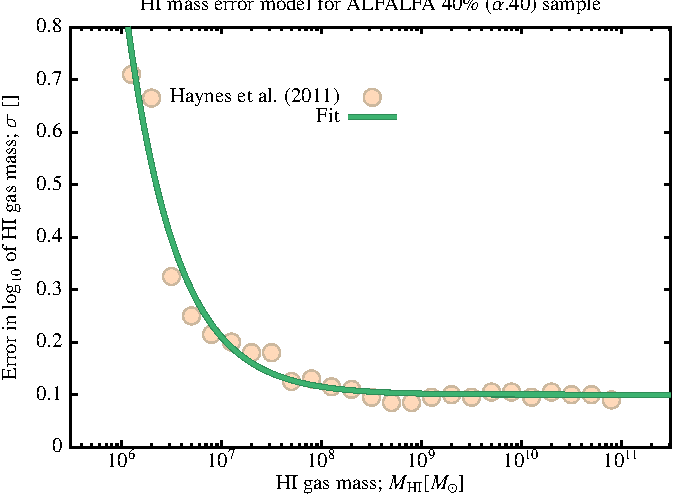
\includegraphics[width=85mm,trim=0mm 0mm 0mm 4mm,clip]{Plots/DataAnalysis/alfalfaHIMassErrorModel.pdf}
 \caption{The observational random error in galaxy HI mass as a function of HI mass for the ALFALFA survey. Points show the errors reported by \protect\cite{haynes_arecibo_2011}, while the line shows a simple functional form fit to these errors.}
 \end{center}
 \label{fig:ALFALFAErrorModel}
\end{figure}

Additionally, HI mass estimates can be affected by HI self-absorption for highly inclined galaxies. \cite[][see also \protect\citealt{zwaan_hipass_2005}]{zwaan_h_1997} estimate that this effect would lead to a mean underestimation of HI masses by a factor $1.1$ for a randomly oriented galaxy sample. Therefore, a value of $-0.0414$ for the systematic parameter {\normalfont \ttfamily [alfalfaHiMassFunctionZ0.00MassSystematic0]} is recommended.
